\label{prelim}
The human operator is modeled as a set of links corresponding to the following body parts: upper arm, lower arm and hand combination, upper torso, lower torso, upper leg, lower leg and foot combination, and neck. While the model may be made more complex, such as including separate links for hands and feet, these joints correspond closely to those controllable by a humanoid robot, so this parsimonious model suffices. Additionally, body parts with small masses and ranges of motions have negligible effect on the CoM beyond the resolution of the Wii Balance Board.

Joints $\mathcal{J}$ are indexed $i = 1,\hdots, N$ with corresponding position in the horizontal frame $r_i \in \mathbb{R}^2$. Note, while in reality, $r_I\in \mathbb{R}^3$, the measurements of CoM from the Wii are only in $\mathbb{R}^2$, so the vertical component of the position is discarded. Given a limb with proximal joint $i$ and distal joint $j$, each limb is modeled as a thin rod link labeled as $(i,j)$. In this context, proximal refers to the limb joint closest to the torso, and distal refers to the joint furthest from the torso. This link has mass $m_{ij}$, length $L_{ij} = \|r_{j}-r_i\|$, and location of center of mass located along the length of the link, distance $l_{ij}=\rho_{ij} L_{ij}$ from the proximal joint. See Figure \ref{fig:humanmodel} for a visual representation. The set of all links used to model the human are given by the set $\mathcal{L}$, and we use the notation $(i,j) \in \mathcal{L}$ to denote that a link exists in our model that connects joint $i$ to joint $j$.

In this setup, the Kinect sensor measures the joint positions in the horizontal frame, $r_i \in \mathbb{R}^2$, and the wii balance measures the CoP of the human in the horizontal frame. Similar to \cite{gonzalez2012estimation,cotton2011estimation}, this work assumes the human operator is static or moving slowly during training. This assumption guarantees that the CoP measured by the Wii balance board is approximately the same as the CoM. 


\begin{figure}
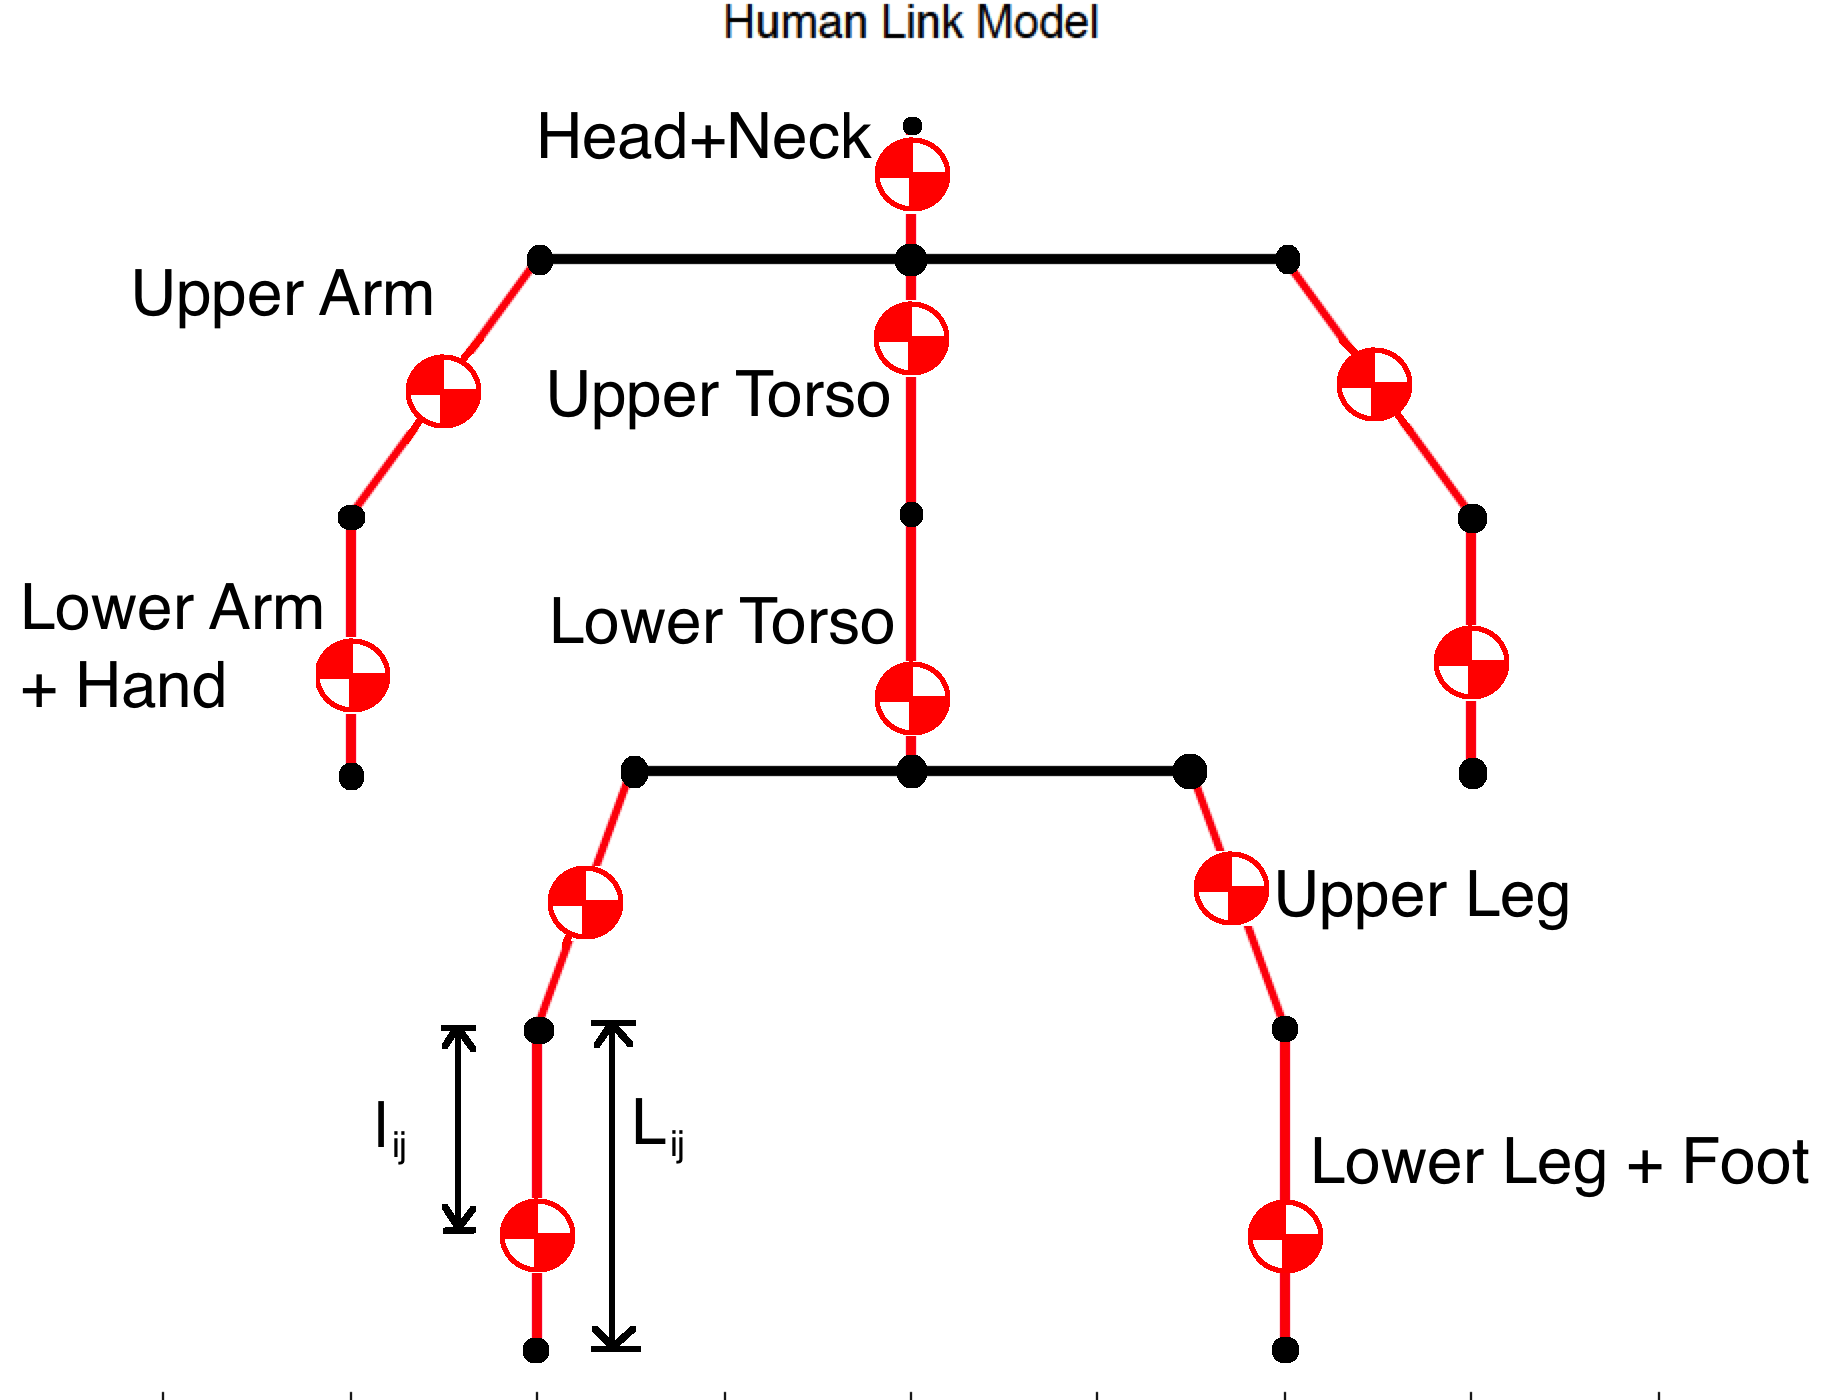
\includegraphics[width=0.9\columnwidth]{figures/skeleton3.png}
\caption{Chain approximation model of a human.}
\label{fig:humanmodel}
\end{figure}

Using this representation, the CoM  can be predicted as
\begin{equation}
\text{CoM} = \frac{1}{M}\sum_{(i,j)\in\mathcal{L}} m_{ij}(1-\rho_{ij})r_i + m_{ij}\rho_{ij}r_j
\end{equation}
where $M$ is the total mass of the human. Alternatively, 
\begin{equation}
\text{CoM} = \frac{1}{M}\sum_{(i,j)\in\mathcal{L}} m_{ij} r_i + m_{ij}\rho_{ij}(r_j - r_i) \label{eq:comSum}
\end{equation}
Consider a na\"ive method of solving for $m_{ij}$, $\rho_{ij}$ using least squares. In this case, we rewrite \eqref{eq:comSum} as, 
\begin{equation}
\text{CoM} = [r_1,  r_2 - r_1, \hdots r_i, r_j - r_i, \hdots] \theta \label{eq:comsingle}
\end{equation}
where
\begin{equation}
\theta = [\frac{m_{12}}{M}, \frac{m_{12}}{M}\rho_{12}, \hdots, \frac{m_{ij}}{M}, \frac{m_{ij}}{M}\rho_{ij}, \hdots]^T \nonumber
\end{equation}
%By estimating the parameter vector $\theta$ and observing the joint positions, one may predict the position of the center of mass as well as calculate the inertial parameters.
Then, given $K$ measurements, $k = 1,\hdots, K$, using superscript to denote measurement number, we concatenate \eqref{eq:comsingle} to receive
\begin{equation}
\begin{bmatrix}
\text{CoM}^1\\
\vdots \\
\text{CoM}^k \\
\vdots \\
\text{CoM}^K
\end{bmatrix}
= 
\begin{bmatrix}
r_1^1,  r_2^1 - r_1^1, \hdots r_i^1, r_j^1 - r_i^1, \hdots  \\
\vdots \\
r_1^k,  r_2^k - r_1^k, \hdots r_i^k, r_j^k - r_i^k, \hdots  \\
\vdots \\
r_1^K,  r_2^K - r_1^K, \hdots r_i^K, r_j^K - r_i^K, \hdots 
\end{bmatrix}
\theta
\label{eq:com}
\end{equation}
For convenience let $Q$ stand for the matrix in \eqref{eq:com}. In the case that a joint is shared by two or more links, i.e. $\exists i,j,k$ s.t. $\{(i,k),(k,j)\} \in \mathcal{L}$, as is the case in the human model, the matrix $Q$ has redundant columns and therefore is ill-conditioned. Regardless of the number of observations, one cannot solve for $\theta$ using least squares. 
This is due to an inherent observability problem when using only static observations. That is to say, when observing the center of mass during only static positions, it is impossible to delineate both how much a link weighs and where the center of mass lies along the link simultaneously. There exists a null space in which a change in the mass of a link coupled with a movement of the center of mass will result in identical center of mass observations. 
The formulations in \cite{gonzalez2012estimation, cotton2011estimation} use only static position measurements and therefore suffer from the same problem of observability. 
